\section{Structured Assurance Case Metamodel}
\label{sec:sec2}
The \textit{Structured Assurance Case Metamodel} (SACM) is standardised by the Object Management Group (OMG). The metamodel is used for the purpose of \textit{System Assurance}, which involves building accurate, comprehensive and defensible arguments regarding systems safety and/or security. SACM captures not only fundamental concepts in the process of \textit{System Assurance} such as \textit{Claim}s and the relationships between \textit{Claim}s, it also captures concepts such as \textit{Artifact}s and \textit{Terminologi}es, in the sense that supporting evidence and information involved in the argument can be expressed in greater precision. 

\subsection{SACM Overview}
In overview, SACM is organised in five packages, as illustrated in Figure \ref{fig:overview}. The \textit{Base} package provides the foundation of SACM, which will be discussed in Section \ref{sec:basePack}. The \textit{Argumentation} package captures the concepts used in arguing system properties (such as safety and/or security)\footnote{System properties refer to the safety and/or security in the context of this paper, hereafter.}, which will be discussed in Section \ref{sec:argPack}. The \textit{Terminology} package captures the concepts used in expressing the arguments regarding system properties, which will be discussed in Section \ref{sec:termPack}. The \textit{Artifact} package captures the concepts used in providing evidence for the arguments made for system properties. The \textit{Artifact} package will be discussed in Section \ref{sec:artiPack}. Finally, the \textit{AssuranceCase} package captures the concepts in \textit{System Assurance}, which combines all the elements in other SACM packages to form a \textit{System Assurance Case}. The \textit{AssuranceCase} package will be discussed in Section \ref{sec:acPack}.
\begin{figure}
	\centering
	\includegraphics[width=0.6\linewidth]{fig/Overview.eps}
	\caption{Packages of SACM}
	\label{fig:overview}
\end{figure}

\subsection{SACM Base Package}
\label{sec:basePack}
The \textit{Base} package captures the foundational concepts of SACM, the structure of the \textit{Base} package is shown in Figure~\ref{fig:base}. The base element of all SACM elements is \textit{Element}. Its direct children are \textit{LangString}, \textit{MultiLangString} and \textit{SACMElement}.
\begin{figure}
	\centering
	\includegraphics[width=1\linewidth]{fig/Base.eps}
	\caption{Packages of SACM}
	\label{fig:base}
\end{figure}

 \textit{LangString} is used as an equivalence to \textit{String} in broad terms, except it provides the addtional feature \textit{+lang} which allows the users to define what language is used in the \textit{LangString}. \textit{ExpressionLangString} is used to not only record a \textit{String} in SACM, but also refer to its corresponding \textit{Expression} organised in a \textit{TerminologyPackage}. The usage of \textit{ExpressionLangString} is discussed in Section~\ref{}. \textit{MultiLangString}, as its name suggests, is used to express the same semantics using different languages. For example, to express 'hazard' in both English and German, the user can create a \textit{MultiLangString} with two \textit{LangString}, like shown in Figure~\ref{fig:mulitiLang}.
\begin{figure}
	\centering
	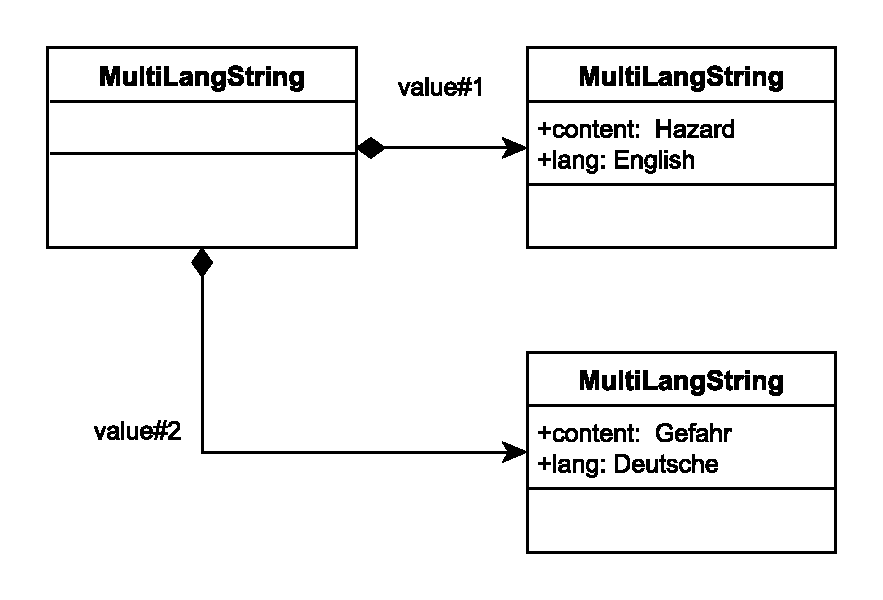
\includegraphics[width=0.5\linewidth]{fig/MultiLangString.eps}
	\caption{Packages of SACM}
	\label{fig:mulitiLang}
\end{figure}
The \textit{MultiLangString} can then be associated to other SACM elements to denote the same meaning. What is more important than multiple natural language support is the support for computer languages. We envision that in the future, system assurance can benefit from automation, by using which system assurance can be partially automated. In this case, \textit{MultiLangString} can be used to hold both natural languages and computer languages (e.g. formal languages) to support automated proving of argumentation. 

\textit{SACMElement} is an abstract element which lays the foundation of all SACM elements. \textit{SACMElement} can record a \textit{+gid}, which stands for \textit{global identification}, for each \textit{SACMElement}, within the same root \textit{Assurance Case}, should have an unique id. \textit{SACMElement} is also able to refer to (or 'cite') other \textit{SACMElement}s, which is useful for implicit references discussed in Section \ref{}. The \textit{citedElement} and \textit{isCitation} properties are used for this purpose. A \textit{SACMElement} can also be abstract, denoted by the \textit{isAbstract} property. A \textit{SACMElement} can also be an \textit{abstractForm} of another, which is discussed in Section \ref{}. 

\textit{ModelElement} further refines \textit{SACMElement} which contains a \textit{name} and a set of \textit{UtilityElement}s. A \textit{ModelElement} can contain a \textit{Description} describe its contents. Like previously mentioned, a \textit{Description} can be expressed in any language via its usage of \textit{MultiLangString}. A \textit{ModelElement} can also contain an \textit{ImplementationConstraint}, in some cases, validation rules and/or queries to models are needed for specific \textit{ModelElement}s, \textit{ImplementationConstraint} can be used to specify such constraints in computer languages (e.g. Object Constraint Language~\cite{}). A \textit{ModelElement} can also contain a number of \textit{Note}s, to hold additional information rather than descriptions. Finally, a \textit{ModelElement} can also contain a number of \textit{TaggedValue}s, which are essentially \{key, value\} pairs. \textit{TaggedValue} can be considered as an extension mechanism to allow the users to associate additional features to a \textit{ModelElement} (other than the features modelled in the current version of SACM\footnote{Version 2.0 as of April, 2018}).

The \textit{Base} package also defines the \textit{ArtifactElement}, in the sense that all elements that extend \textit{ArtifactElement} are considered to be \textit{Artifact}s. The reason for this is discussed in Section~\ref{}. 

In summary, the \textit{Base} package lays the foundation for SACM, it provides facilities not to only express assurance cases (to be precise, assurance case models) in natural language, but also in computer languages. The \textit{Base} package also provides a number of \textit{UtilityElement}s so that the user can use them to describe \textit{ModelElement}s as precisely as possible.

\subsection{SACM Argumentation Package}
\label{sec:argPack}
The \textit{Argumentation} Package captures the concepts required to model structured arguments regarding system properties. The structure of the \textit{Argumentation} package is shown in Figure~\ref{fig:arg}. 

\begin{figure}
	\centering
	\includegraphics[width=1\linewidth]{fig/Argumentation.eps}
	\caption{Packages of SACM}
	\label{fig:arg}
\end{figure}
The root element of the \textit{Argumentation} package is the \textit{ArgumentationElement}, which is a direct child of \textit{ArtifactElement} in the \textit{Base} package. This implies that all elements in the \textit{Argumentation} package are also considered to be artifacts. 

To promote modularity, argumentations are organised in \textit{ArgumentPackage}s. \textit{ArgumentationPackage} can contain a number of \textit{ArgumentationElement}, which can either be \textit{ArgumentPackage}s (and their children) or \textit{ArgumentAsset}s. \textit{ArgumentPackageInterface} 

\subsection{SACM Terminology Package}
\label{sec:termPack}

\begin{figure}
	\centering
	\includegraphics[width=1\linewidth]{fig/Terminology.eps}
	\caption{Packages of SACM}
	\label{fig:term}
\end{figure}
\subsection{SACM Artifact Package}
\label{sec:artiPack}

\begin{figure}
	\centering
	\includegraphics[width=1\linewidth]{fig/Artifact.eps}
	\caption{Packages of SACM}
	\label{fig:arti}
\end{figure}
\subsection{SACM AssuranceCase Package}
\label{sec:acPack}

\begin{figure}
	\centering
	\includegraphics[width=1\linewidth]{fig/AssuranceCase.eps}
	\caption{Packages of SACM}
	\label{fig:ac}
\end{figure}